\documentclass[a4, 11pt]{article}
\usepackage{inputenc}[utf-8]
\usepackage{newtx}
\usepackage{float}
\usepackage{graphicx}
\usepackage{geometry}
\usepackage{listings}
\usepackage{courier}
\usepackage{xcolor}

\definecolor{codegreen}{rgb}{0,0.6,0}
\definecolor{codegray}{rgb}{0.5,0.5,0.5}
\definecolor{codepurple}{rgb}{0.58,0,0.82}

\lstdefinestyle{mystyle}{   
    commentstyle=\color{codegreen},
    keywordstyle=\color{magenta},
    numberstyle=\tiny\color{codegray},
    stringstyle=\color{codepurple},
    basicstyle=\ttfamily\footnotesize,
    breakatwhitespace=false,         
    breaklines=true,                 
    captionpos=b,                    
    keepspaces=true,                                   
    showspaces=false,                
    showstringspaces=false,
    showtabs=false,                  
    tabsize=2
}

\lstset{style=mystyle}

 \geometry{
 a4paper,
 left=25mm,
 top=25mm,
 }
\title{Hate Speech Detection - TiMBL}
\author{Ravi Regulagedda, Jieli Liu, Ugonna Virginia Ahumibe}
\date{}

\begin{document}
\maketitle

Initial Accuracy with no hyper-parameter tuning: 70.5451\%
\begin{figure}[H]
\center
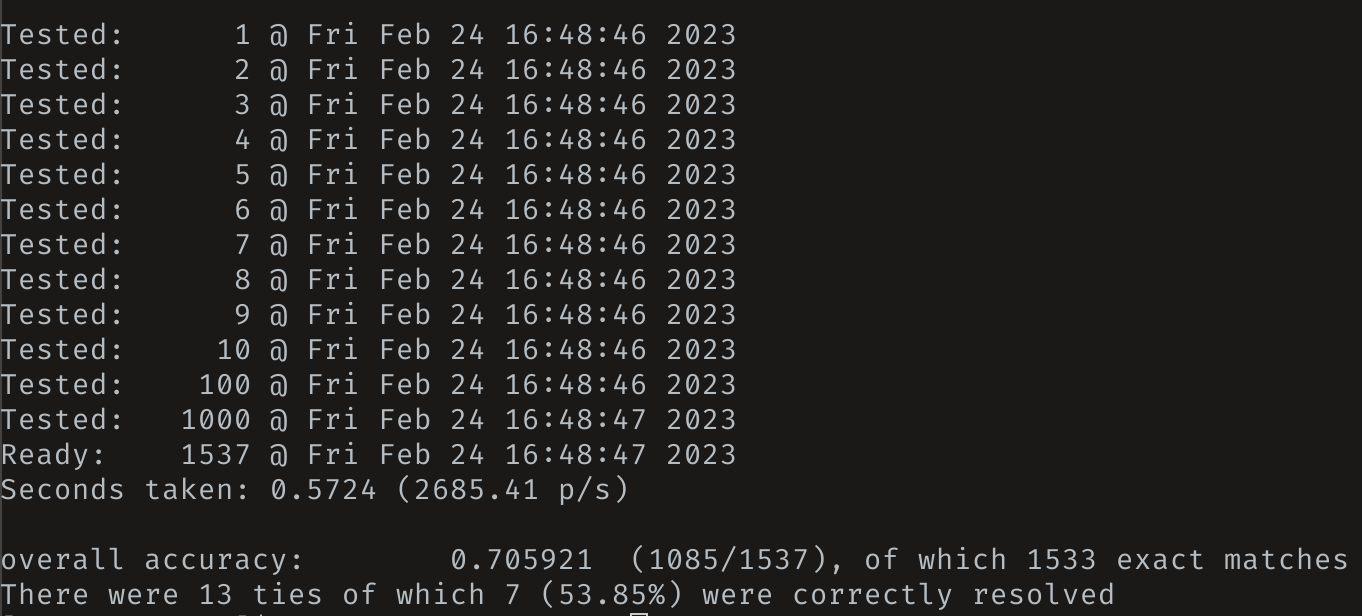
\includegraphics[scale=0.4]{baseline.png}
\caption{Result showing the baseline accuracy}
\end{figure}
After many tests the best results were achieved with \lstinline{-a 4}. Every other parameter had no affect on the data, or produced worse results. The final accuracy was an improvement of 0.1\% bringing the final accuracy upto 70.6571\%.

In some cases, setting parameters like \lstinline{-k 7} etc., improved the performance but they never gave a better performance than the above parameter. Another interesting observation was the test set and dev set had different optimal parameters. The dev set had greatest accuracy at \lstinline{-a 3 -k 7 -b 9}. For these parameters, the test set had a lower accuracy than the baseline at 70.3\%

The output showing the accuracy for the test set is below.
\begin{figure}[H]
\center
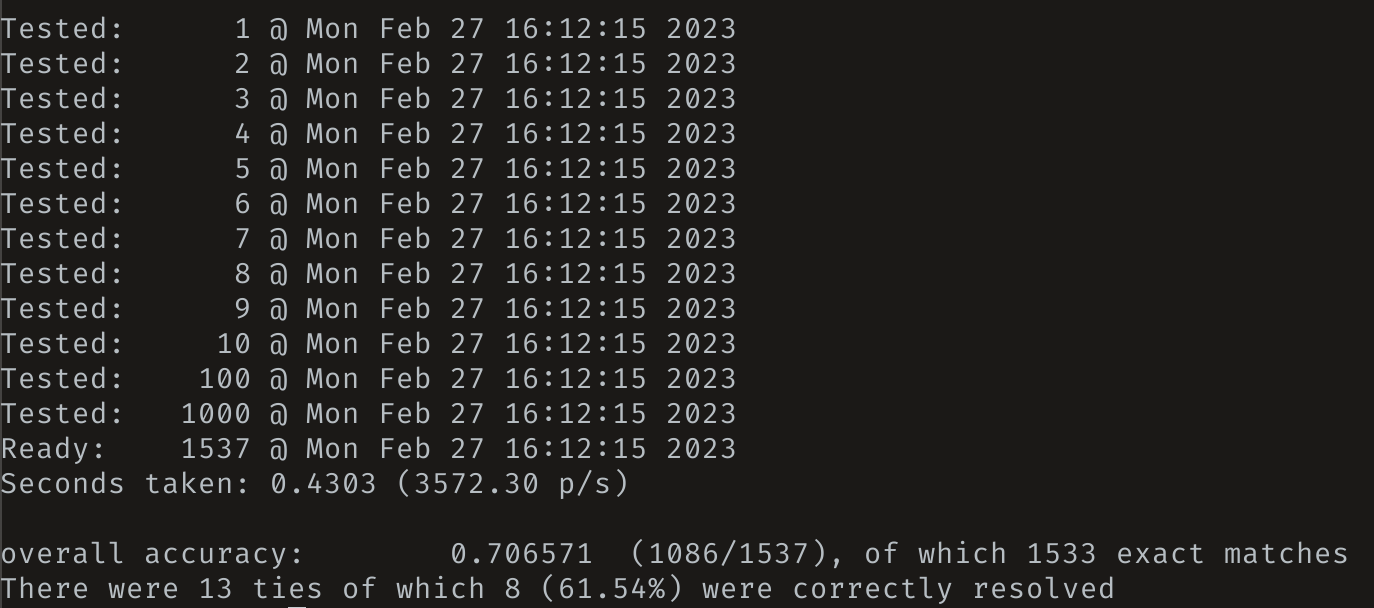
\includegraphics[scale=0.4]{final.png}
\caption{Result showing the baseline accuracy}
\end{figure}
\end{document}